\documentclass[12pt,a4paper]{article}
\usepackage[colorlinks=true, urlcolor=blue, linkcolor=red]{hyperref}
\usepackage{amsmath, amssymb, amsthm, algorithm, booktabs, listings}
\usepackage[dvipsnames,usenames]{xcolor}
\usepackage[noend]{algpseudocode}
\usepackage{tikz}
\usepackage{fancyhdr}
\usepackage{geometry}
\newgeometry{top=2cm, bottom=2cm, left=1.5cm, right=1.5cm}
\usepackage[shortlabels]{enumitem}
\usepackage{cleveref}
\usepackage{mdframed}
\usepackage[most]{tcolorbox}
\hypersetup{citecolor=blue}
\usepackage{times}
\theoremstyle{definition}
\newtheorem{definition}{Definition}[subsection]
\newtheorem{statement}{Statement}[subsection]
\usepackage[backend=biber,style=alphabetic,sorting=ynt]{biblatex}
\hypersetup{linkcolor=black}
\addbibresource{references.bib}
\pagestyle{fancy}
\defbibheading{blueboxed}{%
  \begin{tcolorbox}[colframe=blue!50!black, colback=blue!20]
    \section{References}
  \end{tcolorbox}
}

\newcommand{\bluebox}[1]{%
  \begin{tcolorbox}[colframe=blue!50!black, colback=blue!20]
    #1
  \end{tcolorbox}%
}

\newcommand{\purplebox}[1]{%
  \begin{tcolorbox}[colframe=violet!80!black, colback=violet!20]
    #1
  \end{tcolorbox}%
}

\newcommand{\pinkbox}[2]{%
  \begin{tcolorbox}[colframe=magenta!50!black, colback=magenta!20, title={#1}]
    #2
  \end{tcolorbox}%
}

\newcommand{\bluebigbox}[2]{%
  \begin{tcolorbox}[colframe=blue!50!black, colback=blue!20, title={#1}, toptitle=5pt, bottomtitle=5pt]
    #2
  \end{tcolorbox}%
}

\DeclareRobustCommand{\hlit}[1]{\colorbox{yellow}{\textit{#1}}}
\DeclareRobustCommand{\hl}[1]{\colorbox{yellow}{#1}}
\DeclareRobustCommand{\ghl}[1]{\colorbox{green}{#1}}
\newcommand{\bs}{\textbackslash}
\newcommand{\boxtxt}[1]{\boxed{\text{#1}}}

\tcbuselibrary{listings}
\newtcblisting{shuncode}{
    listing only,
    listing options={
        language=C,
        basicstyle=\ttfamily\small,
        keywordstyle=\color{blue},
        commentstyle=\color{green!50!black},
        stringstyle=\color{red}
    },
    colback=cyan!10,
    colframe=cyan!80!black,
    boxrule=2pt,
    left=0pt,
    right=0pt,
    top=0pt,
    bottom=0pt,
    boxsep=0pt,
    arc=5pt,
    enhanced
}

\lhead{Computer Networks}
\chead{Chapter 1 Summary}
\rhead{Shun (@shun4midx)}

\begin{document}
\begin{center}
  {\Large \bf Computer Networks: Chapter 1 Summary}\\[8pt]
  \textbf{Author:} Shun (@shun4midx)
\end{center}

\bluebox{\section*{Basic Definitions}}
\purplebox{\subsection*{Overview}}
\noindent The internet is a ``network of networks'' \textbf{(Interconnected ISPs, i.e. Internet Service Providers)}, where a \textbf{network} is a collection of devices, routers, and links \emph{managed by an organization}
\vspace{0.5em}\begin{itemize}
    \item \textbf{Hosts} = End systems
    \item \textbf{Packet Switches} = Forward packets (chunks of data), e.g. \hlit{routers, switches}
    \item \textbf{Communication Links}: E.g. \hlit{fiber, copper, radio, satellite}; \hl{\textbf{transmission rate} = \emph{bandwidth}} in bps
    \item \textbf{Internet Services}: \textbf{Infrastructure} to provide services to apps (e.g. web, email, streaming, etc), \textbf{programming interface} such as \emph{hooks} to ``connect'' and \emph{service}
\end{itemize}

\pinkbox{Protocol}{
    \textbf{Protocols} define the \textbf{format, order} of \textbf{messages sent and received} among network entities, and \textbf{actions taken} on message transmission, receipt.
}

\vspace{1.0em}\bluebox{\section*{Network Edge}}
\purplebox{\subsection*{Access Networks}}
\noindent \textbf{Access networks} are how end systems connect to \textbf{edge routers}. 

\vspace{0.5em}\begin{itemize}
    \item \textbf{HFC} (Hybrid Fiber Coax): A network of \emph{fiber} (to the \textbf{neighborhood node}) and \emph {shared coax} (to homes) attaches homes to the ISP router at the \textbf{cable headend}; \hl{Higher downstream transmission} \hl{compared to upstream}
        \begin{itemize}
            \item Uses \textbf{cable-based access} via \textbf{FDM} (frequency division multiplexing), i.e. different channels are transmitted in different frequency bands
        \end{itemize}
    \item \textbf{DSL} (Digital Subscriber Line): Uses existing \hlit{telephone line} to central office \textbf{DSLAM} (Data connects to internet, voice connects to telephone net); Higher downstream transmission compared to upstream
\end{itemize}

\noindent There are two main kinds of \textbf{wireless access networks} that connect end systems to router:
\begin{itemize}
    \item \textbf{WLANs} (Wireless Local Area Networks): Typically within or around building, e.g. \hlit{Wi-Fi}. Can have low or high transmission rates.
    \item \textbf{Wide-Area Cellular Access Networks}: Provided by \emph{mobile, cellular network operator}, typically medium transmission rate (around \textbf{tens of Mbps}), e.g. \hlit{4G/5G cellular networks}
\end{itemize}

\pinkbox{Examples of Access Networks}{
    \begin{itemize}
        \item \textbf{Home Access:} DSL, HFC/Cable
        \item \textbf{Wide-area Wireless:} 4G LTE, 5G NR.
    \end{itemize}
}

\pinkbox{Local Networks (LANs, Inside Premises)}{
    \begin{itemize}
        \item \textbf{Home LAN:} Wi-Fi + Ethernet switch + NAT/firewall (often one gateway).
        \item \textbf{Enterprise LAN:} Switched Ethernet access + Managed Wi-Fi.
    \end{itemize}
}

\purplebox{\subsection*{Physical Media Links}}
\pinkbox{Physical Media Links}{
    A \textbf{physical link} is what lies between transmitter and receiver
    \begin{itemize}
        \item \textbf{Guided}: Signals propagate in \textbf{solid media}, e.g. \hlit{twisted pair/TP} (two insulated copper wires), \hlit{coaxial cable} (bidirectional, two concentric copper conductors), \hlit{fiber optic cable} \hl{(high speed operation, low error)}.
        \item \textbf{Unguided}: Signals propagate \textbf{freely}, e.g. \textbf{radio}, such as \hlit{Wi-Fi, wide-area, bluetooth,} \hlit{terrestrial microwave, satellite}
    \end{itemize}
}

\vspace{1.0em}\bluebox{\section*{Network Core}}
\purplebox{\subsection*{Packet Switching and Circuit Switching}}
\noindent There are two key network-core functions:
\vspace{0.5em}\begin{itemize}
    \item \hl{\textbf{Forwarding} (i.e. \emph{switching}): \emph{Local}}, moves packets from router's input link to output link
    \item \hl{\textbf{Routing}: \emph{Global} action}, determines best paths taken by packets
\end{itemize}

\pinkbox{Packet vs. Circuit Switching}{
    \textbf{Packet switching:} Messages $\to$ packets; each hop does \textit{store-and-forward}. It \textbf{queues} your desired packets into a buffer whenever \hl{\textbf{arrival rate $>$ transmission rate}}.
    \begin{itemize}    
        \item \textbf{Pros}: Efficient sharing, good for bursty traffic, no call setup.
        \item \textbf{Cons}: Queueing delay, possible loss under congestion.
    \end{itemize}
    \textbf{Circuit switching:} End-to-end resources reserved for \textbf{call between source and destination}, i.e. you posses the entire line at a time.
    \begin{itemize}
        \item \textbf{Pros}: Predictable performance.
        \item \textbf{Cons}: Idle when unused, setup overhead.
    \end{itemize}
}

\pinkbox{Example Calculation}{
    \textbf{Problem:} Say we have a 1 Gb/s output link, and each user uses 100 Mb/s when active. Each user is active around 10\% of the time. How many users can use this network under circuit-switching and packet-switching? \\

    \textbf{Circuit-Switching:} Each user possesses the \emph{entire line at a time}, so $\frac{1 \text{Gb/s}}{100 \text{Mb/s}} = \boxed{10 \text{ users}}$ \\

    \textbf{Packet-Switching:} Say there are 35 users, then by binomial distribution, the probability that \hl{\textbf{more than 10} (maximum amount which we can share) are active at the same time} is less than $0.0004$. This means, we can hold 35 users with only $0.0004$ of the data not being able to be sent.
}

\vspace{0.5em}\purplebox{\subsection*{Internet Structure}}

\noindent Intuitively, the reasoning is we require all hosts to be able to interconnect with each other, with as few connections as possible. As we cannot have one big global ISP (\textbf{Internet Service Provider}) in practice, we end up creating \textbf{several ISPs}, including \emph{regional ISPs} and other \textbf{``tier-1'' commercial ISPs}, e.g. \emph{AT\&T, NTT}, which regional ISPs connect to. Then, we \hl{interconnect them with \textbf{IXPs (Internet Exchange Points)}}. Otherwise, a \textbf{content provider network} (e.g. Google), which is a private network, connects its data center to the Internet, often \hl{\textbf{bypassing most ISPs}}. Hence why we say the internet is a \emph{``network of networks''}.

\begin{figure}[h]
    \centering
    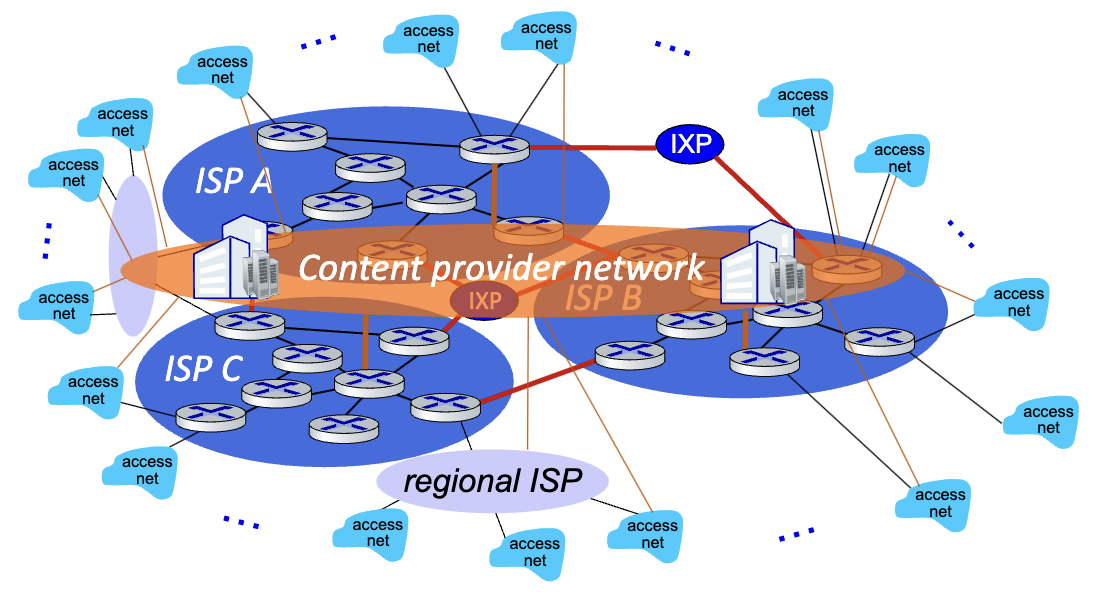
\includegraphics[width=0.5\textwidth]{ch1_img/internet_structure.png}
    \caption{A visual for internet structure.}
    \label{fig:internet_structure}
\end{figure}

\vspace{1.0em}\bluebox{\section*{Performance Loss: Delay and Throughput}}
\purplebox{\subsection*{Packet Delay}}
\noindent There are four main types of packet delay, as better shown in the figure below.
\begin{figure}[h]
    \centering
    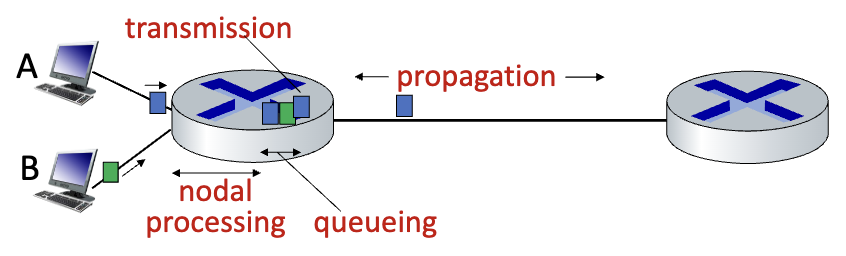
\includegraphics[width=0.44\textwidth]{ch1_img/packet_delay.png}
    \caption{Depiction of the four main sources of packet delay}
    \label{fig:packet_delay}
\end{figure}

\pinkbox{Packet Delay Formula}{
    In general, we have:
    $$
    \hl{\boxed{d_{\text{nodal}} = d_{\text{proc}} + d_{\text{queue}} + d_{\text{trans}} + d_{\text{prop}}}}
    $$

    \begin{itemize}
        \item \ghl{\textbf{Nodal Processing \emph{(Const)}:}} When checking bit errors and determining \emph{output link}; typically within \emph{microsecs}
        \item \textbf{Queueing Delay:} Time waiting at output link for transmission, depends on the congestion level of the router
        \item \textbf{Transmission Delay:} \hl{$d_{\text{trans}} = \frac{L}{R}$}, $L$ = \emph{packet length (bits)}, $R$ = link \emph{transmission rate (b/s)}
        \item \ghl{\textbf{Propagation Delay \emph{(Const)}:}} \hl{$d_{\text{prop}} = \frac{d}{s}$}, $d$ = \emph{length of physical link}, $s$ = \emph{propagation speed} ($\approx 2 \times 10^8$ m/s)
    \end{itemize}
}

\pinkbox{Traffic Intensity (Packet Queueing Delay)}{
    Define $a$ as the average packet \emph{arrival rate}, $L$ as the packet length in bits, and $R$ as the link bandwidth (bit transmission rate). We define the \textbf{traffic intensity} as follows:

    $$
    \frac{L \cdot a}{R} = \frac{\text{arrival rate of bits}}{\text{service rate of bits}}
    $$

    \vspace{1.0em}Usually, traffic intensity could tell us certain info as follows:
    \begin{itemize}
        \item $\frac{La}{R} \approx 0$: average \emph{queueing delay is small}
        \item $\frac{La}{R} \to 1$: average \emph{queueing delay is large}
        \item $\frac{La}{R} > 1$: work arriving $>$ servicable work $\Rightarrow$ infinite delay!
    \end{itemize}
}

\vspace{1.0em}\noindent In real life, we can use \texttt{traceroute <website>} in the terminal to measure internet delay. It will output the time elapsed for each (publically accessible) step required, to reach said website.

\vspace{1.0em}\purplebox{\subsection*{Throughput}}
\pinkbox{Throughput Definition}{\textbf{Throughput} is defined as the \textbf{rate} (bits/time) at which bits are being \textbf{sent} from sender to receiver.}

\noindent In practice, $R_c$ or $R_s$, as demonstrated below, is the bottleneck. In extreme cases, $R$/(number of shared connections) may be the bottleneck. \hl{\textbf{The bottleneck is the minimum rate $R$}}.

\vspace{-1.0em}\begin{figure}[h]
    \centering
    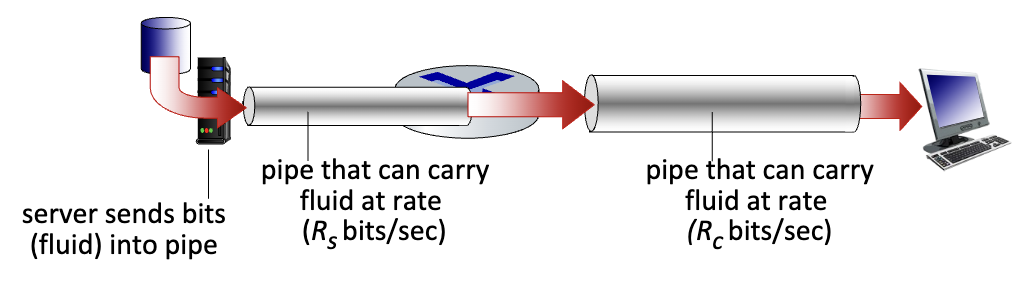
\includegraphics[width=0.65\textwidth]{ch1_img/throughput.png}
\end{figure}

\vspace{1.0em}\bluebox{\section*{Network Security}}
\noindent The main takeaway is the Internet was designed \textbf{without considering adverseries}, so it's \textbf{prone to attacks}.

\vspace{0.5em}\pinkbox{Types of Attacks}{
\begin{itemize}
  \item \textbf{Denial of Service (DoS):} Overwhelm resources to block service
  \item \textbf{Packet Sniffing:} Reads all packets (including passwords) in a network
  \item \textbf{Spoofing:} Injection of packet with false sourcce address
\end{itemize}
}

\pinkbox{Countermeasures}{
\begin{itemize}
  \item \textbf{Cryptography:} Encryption, authentication
  \item \textbf{Integrity Checks:} Signatures to prevent and detect tampering
  \item \textbf{Firewalls} to avoid DoS attacks and filter incoming packets
\end{itemize}
}

\vspace{1.0em}\bluebox{\section*{Protocol Layers and Reference Models}}

\noindent \textbf{Layering Principle:} Modular design; each layer offers services to the layer above and relies on services from the layer below. Then, change in layer service implementation is isolated from other layers.

\vspace{0.5em}\pinkbox{Internet (TCP/IP) model: 5 layers}{
\begin{enumerate}
  \item \textbf{Application:} Supports network applications (e.g. \emph{HTTP, IMAP, SMTP, DNS})
  \item \textbf{Transport:} Process-to-process data transfering (e.g. \emph{TCP, UDP})
  \item \textbf{Network:} Routes datagrams from source to destination (e.g. \emph{IP, routing protocols})
  \item \textbf{Link:} Transfers data between neighboring network elements (e.g. \emph{Ethernet, Wi-Fi, PPP})
  \item \textbf{Physical:} bits ``on the wire''
\end{enumerate}
}

\pinkbox{Encapsulation}{
    As data travels down the stack, each layer \textbf{adds a header}. As data travels up, each layer \textbf{removes its header}. This crates a \textbf{link-layer frame} via what we call \textbf{encapsulation}.
}

\vspace{-1.0em}\begin{figure}[h]
    \centering
    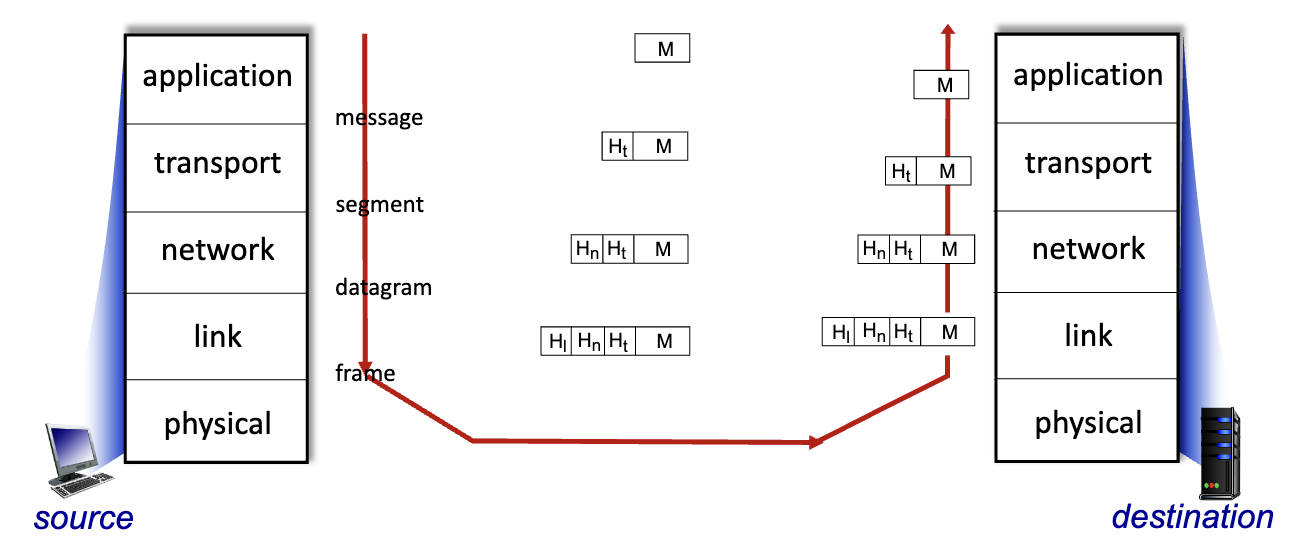
\includegraphics[width=0.65\textwidth]{ch1_img/encapsulation.png}
\end{figure}

\end{document}